%!TEX encoding=UTF-8 Unicode
\chapter{Analyzing Fine Grained Memory Traces}

\gls{Tabarnac} traces contain two parts: informations about the data structures and the actual trace.
For small applications with a limited number of data structures, it is relatively easy to present the first kind of information.
The actual trace is spread over three dimensions: threads, pages and type of accesses, however, this last one can only take two values (read or write).
Finding a meaningful and comprehensive representation for such data is slightly more complex but it is still doable.
\gls{Moca} traces are way more generic.
Indeed, they contain the same meta data and the actual trace also provides information about time and \gls{CPU} location.
Therefore, these traces are spread over five dimensions: time, addresses, type of access, thread and \gls{CPU} location.
Furthermore some of these dimensions can be seen from several point of view, for instance we can look either at the physical or virtual address space.
As we are not used to visualize things in more than three dimensions, to analyze these traces, we must provide the user with a way to navigate through different representations.
Additionally, we need to help the user identify and focus on the important parts.

The contribution presented in this chapter consists in two different methods to analyze \gls{Moca} traces:
\begin{itemize}
    \item The first method relies on \gls{Framesoc}~\cite{Pagano14frameSoC}, an existing generic trace management tool, and more specifically one plugin called \gls{Ocelotl}~\cite{Dosimont14Ocelotl} that provide aggregated views of a trace.\\
        We have implemented an importer to analyze \gls{Moca} traces in \gls{Framesoc} that is distributed on Github under GPL License:\\
        \url{https://github.com/dbeniamine/framesoc\_importer\_moca}.\\
        \DB{Distribute properly and fix moca importer}
        The proposed visualizations are presented in a Research Report~\cite{Beniamine15Memory}.
    \item The second method relies on \gls{R}, it is an ongoing work, publicly available online at:
        \url{https://github.com/dbeniamine/Moca\_visualization}
\end{itemize}

This chapter is organized as follows: first we present our analysis of \gls{Moca} traces with \gls{Framesoc} and \gls{Ocelotl} with an example and discuss the limits of this method in \sect{visu-first}.
Then we propose a second, more flexible approach based on \gls{R} in \sect{visu-second}.
Finally we present some perspective of improvement of these analysis and our conclusions in \sect{visu-cncl}.


\section{Interactive visualization of aggregated traces}
\label{sec:visu-first}

As \gls{Moca} traces are spread over five dimensions and as the address space of an application can be quite large, we need a way to navigate easily in the trace and highlight interesting parts.
Consequently, we are looking for a tool that is able to run high level analysis with for instance the ability to spot anomalies.
While several generic trace manager tools such as \gls{HPCToolkit}~\cite{Adhianto10HPCTOOLKIT} are able to import generic traces, we decided to use \gls{Framesoc}~\cite{Pagano14frameSoC}.
This decision was mainly motivated by one of \gls{Framesoc} visualization tool, \gls{Ocelotl}~\cite{Dosimont14Ocelotl} that is designed specifically to aggregate similar parts of a trace and identify anomalies.

\subsection{FrameSoc and Ocelotl}

\gls{Framesoc} is a generic trace management infrastructure, it provides importers to read traces from many different format.
From its point of view a trace consists on five sets:
\begin{enumerate}
    \item Some meta data about the trace, such as the name of the trace, the application traced, the number of \glspl{CPU} used, the \gls{OS} and so on\ldots
    \item A set of \emph{Event Producers}: which are entities able to produce some \emph{Events}.
        For classic performance traces the Event producers are the \glspl{CPU}, threads or processes.
    \item A set of \emph{Events Types} used to classify the possible events.
        \gls{MPI} function calls and system calls are two usual event types.
    \item A set of \emph{Events}, \emph{Variables} and \emph{States} that form the actual trace.
        For instance in a classic trace, a call to a call to \texttt{MPI\_Send} could be an event, and a \gls{CPU} could be in \emph{idle} state after a call to \texttt{MPI\_Receive}.
        Variables are used to represent values that evolves as the time passes.
    \item A set of \emph{Links} that can be used to represent causality between events, variables and states.
\end{enumerate}

To analyze a trace from an unknown format in \gls{Framesoc}, we need to write an importer which is a relatively simple task.
Indeed \gls{Framesoc} is implemented as an Eclipse plugin, consequently an importer is a small piece of java code that read a trace file, create the sets described above and store them in a database, using \gls{Framesoc} \gls{API}.
The main challenge in the writing of an importer is to figure out how to represent the trace in \gls{Framesoc} internal model.

\gls{Framesoc} provides several functionalities to explore a trace such as filtering events by type, name, focusing on a time frame.
Additionally it has a multi view representation which means that several views of the trace can be opened at the same time and synchronized.
For instance a user can start inspecting a trace with a Gantt chart, focus on a small part and then look at a pie chart of the event distribution in this subset of the trace.
\gls{Framesoc} is optimized to make such analysis as smooth as possible.

\gls{Ocelotl}~\cite{Dosimont14Ocelotl} is an analysis tool for \gls{Framesoc}.
This tool is particularly interesting for us as it provides an aggregated overview of a trace.
The idea behind \gls{Ocelotl} is that a trace with too many entities (events or event producers) is not understandable, consequently, it should be analyzed with a \emph{systemic approach}.
This means considering the whole trace as a system and finding a macroscopic representation of that system that contains an amount of information understandable by a human.
To do so, it uses an aggregation methodology proposed by Lamarache-Perrin~\cite{Lamarche_Perrin14Agregation} and adapted for trace analysis.
This methodology cuts the trace into small slices over the two dimensions: time and space (event producers).
Then it considers each possible partition, benefiting from the structure enforced on time and space to reduce the number of possibilities.
For instance, merging two slices that are not continuous over time is not allowed as it would not be meaningful.
In addition, it uses a parameter $p<[0,1]$ that controls the trade-off between information loss and data reduction and find the optimal partition for this parameters.
Once the first visualization is generated, \gls{Ocelotl} provide the ability to explore the trace (zoom, use \gls{Framesoc} filters \ldots) and change the $p$ parameter.
The usual workflow with \gls{Ocelotl} is starting with a high $p$, where the trace is mostly aggregated, zoom on anomalies or interesting parts and decreasing $p$ to understand more precisely what phenomena we are observing.

\begin{figure}[htb]
    \centering
    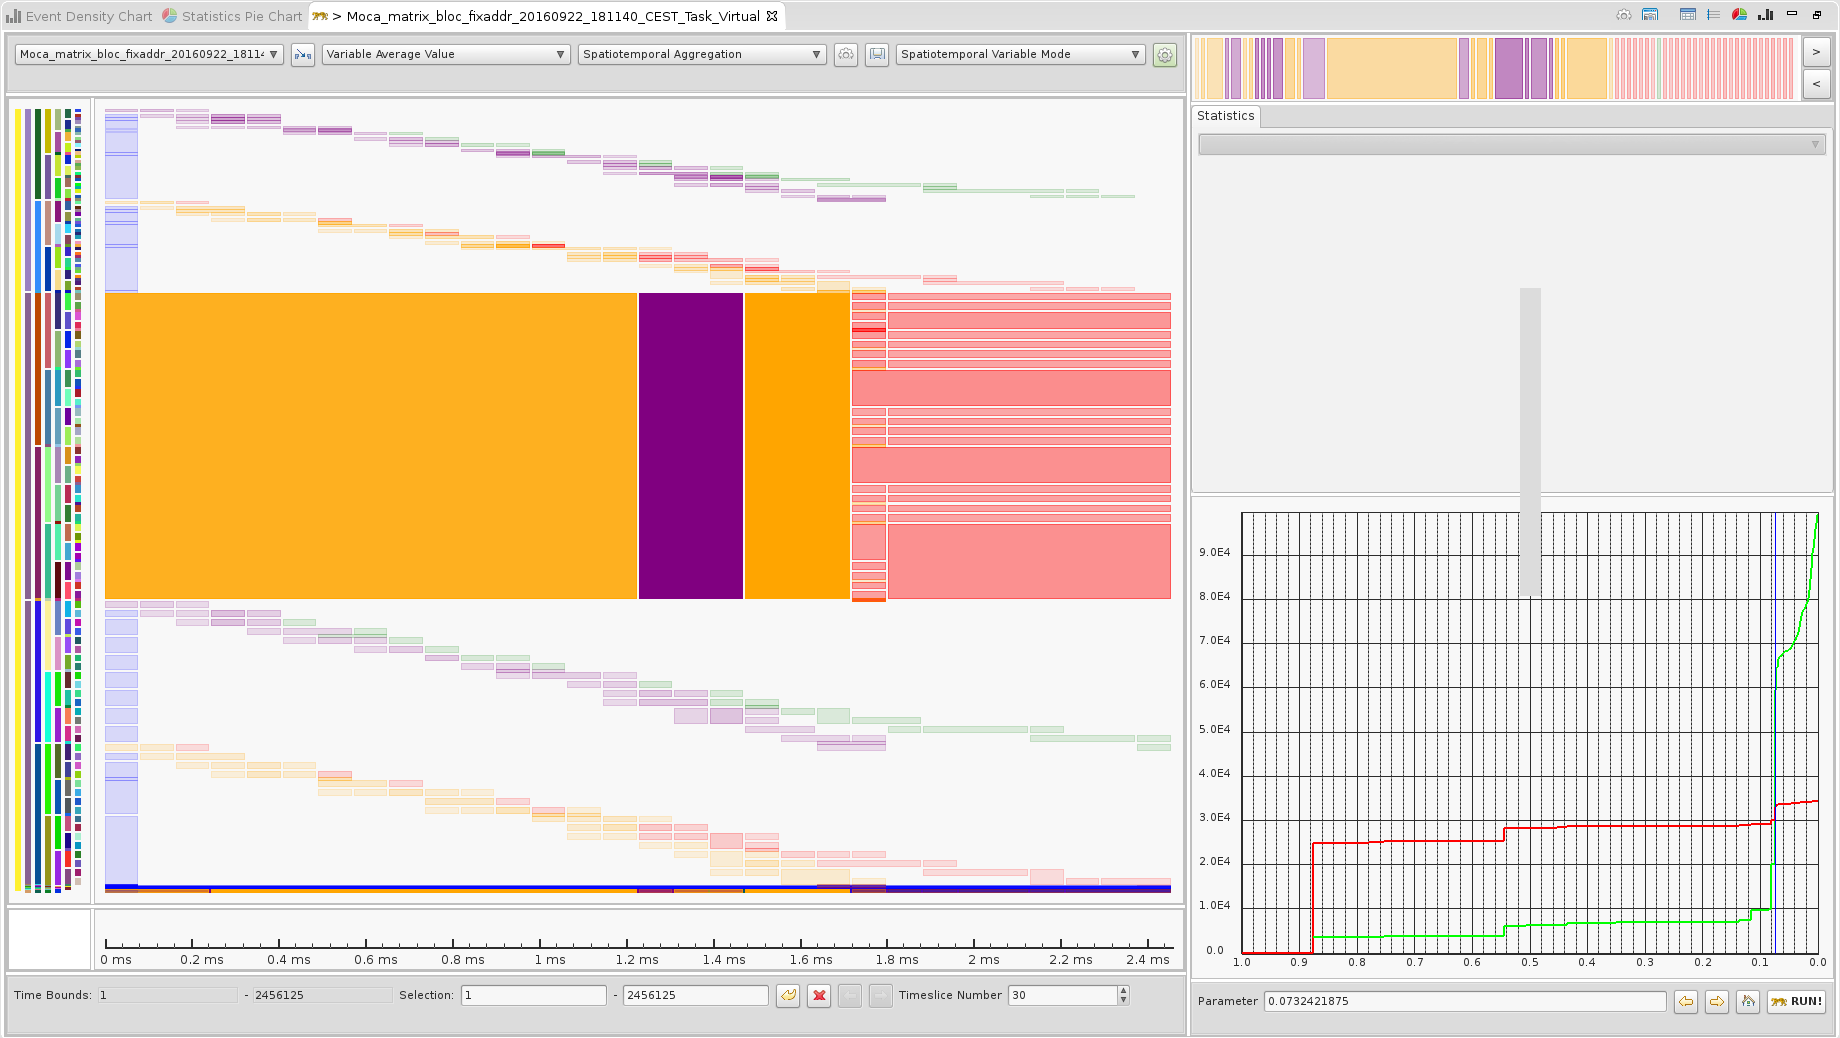
\includegraphics[width=\linewidth]{ocelotl/overview.png}
    \caption{Screenshot of Ocelotl.}
    \label{fig:ocelotl-overview}
\end{figure}

\fig{ocelotl-overview} is a screenshot of \gls{Ocelotl}, showing on the main pane an overview of an example trace, aggregated over time and space (memory addresses).
The X-axis represents time and the Y-axis represent the memory space, we can see on the left that the Y-axis is organized hierarchically.
This hierarchy is used to reduce the number of possible aggregations, indeed, for one level of the hierarchy, \gls{Ocelotl} can only merges two event producers if they have the same parent.
Without any a priory knowledge of the trace application, we can distinguish three phases on this visualization: a short initialization (blue column at the beginning), the main execution with some pattern change around the two third of the execution.
The top right pane shows a summary of the trace aggregate only over the time.
On this summary, the initialization is a bit less visible.
Finally the bottom right pane shows a comprehensive visualization of the information versus complexity gain depending on the value of $p$.
The red curves show the information gain and the green one the complexity gain.
The current value of $p$ is showed by a blue vertical line, and displayed in a text block under the curve.
We can set the $p$ parameter either by clicking the curve or by entering the requested value inside the text block.
At this point the user could zoom in a subpart of the trace by selecting it, or change the parameter $p$ to disaggregate the visualization.

\subsection{Trace Description}

As explained earlier, \gls{Moca} traces are spread on five dimensions while \gls{Framesoc} is designed for two dimensional traces (time and event producers).
Nevertheless we can use the \emph{event types} of \gls{Framesoc} to represent some of the missing dimensions.
To provide different visualization of the same trace, our importer produces four different \gls{Framesoc} traces with different event types.
For all the traces, the event producers represent the memory addresses, but the two first are based on virtual addresses while the two others physical addresses.

The more event producer there are, the more partitions \gls{Ocelotl} must consider to compute the aggregation.
Yet, \gls{Ocelotl} uses the structure of the event producer hierarchy to reduce the number of allowed partitions, indeed it can only merge event producers that have the same parent.
Consequently we can counterbalance the huge number of event producers by creating an artificial hierarchy in the memory.
We can build a meaningful hierarchy that also adds some semantic to the trace: to do so we create a virtual \emph{Memory Root} event producer that is the parent of all the event producers.
Then, the second level of event producers is composed of the stacks and data structures.
All the addresses that are not in these set, are merged if they are contiguous, creating chunks of continuous addresses which are also second level event producers.
Then, each subsequent level is obtained by splitting the previous one on two or three parts, until we reach at the page level.
The pages are the leaves of this artificial memory hierarchy.
We could divide the pages in cache lines and keep going until the address granularity, but this would generate way more event producer that what \gls{Ocelotl} is able to handle.

For both physical and virtual addressing, our importer creates two different traces.
In the first type of trace, the events and spread on four event types: \texttt{private\_read}, \texttt{private\_write}, \texttt{shared\_read}, \texttt{shared\_write}.
For the second trace, we add to these types the number of the thread responsible of the access, for instance \texttt{private\_read\_T0} for the thread $0$.
As a result we have for both physical and virtual addresses, we have two views one representing the usage of the memory by the threads and one global view presenting the sharing patterns.

Each access is represented by a variable, whose value is the number of threads involved in the access.
Finally, the \gls{CPU} on which the access occurred is stored as an event parameter.

\subsection{Sharing detection}

\begin{figure}[htb]
    \centering
    %!TEX encoding=UTF-8 Unicode
% Palette Dark2 3 colors
\definecolor{ColF}{HTML}{1B9E77}
\definecolor{ColV}{HTML}{D95F02}
\definecolor{ColM}{HTML}{7570B3}



\tikzset{
    % Args: BeginVal, EndVal, Size, label, Color
    pics/access/.style args={#1#2#3#4#5}{
        code={
            \draw[|-|,thick,#5] (0,0) node[pos=0,below=2pt,#5]{#1} -- (#3,0)
            node[pos=1,below=2pt,#5]{#2};
            \node[ColV][anchor=south] at (#3/2,0) {#4};
        }
    },
}
\tikzstyle{mybrace} = [decorate,decoration={brace, mirror,amplitude=1em},thick]

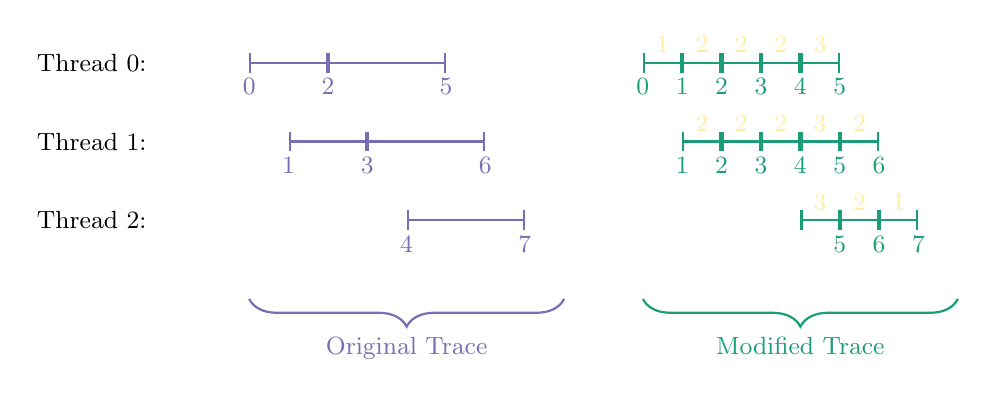
\begin{tikzpicture}[font=\small]
    \node at (-2,0) {Thread 0:};
    \node at (-2,-1) {Thread 1:};
    \node at (-2,-2) {Thread 2:};

    \draw[mybrace,ColM] (0,-3) -- (4,-3) node[pos=.5,below=1em] {Original Trace};
    \draw[mybrace,ColF] (5,-3) -- (9,-3) node[pos=.5,below=1em] {Modified Trace};

    % Moca trace
    \pic at (0,0)       {access={0}{2}{1}{}{ColM}};
    \pic at (1,0)       {access={ }{5}{1.5}{}{ColM}};

    \pic at (0.5,-1)    {access={1}{3}{1}{}{ColM}};
    \pic at (1.5,-1)    {access={ }{6}{1.5}{}{ColM}};

    \pic at (2,-2)      {access={4}{7}{1.5}{}{ColM}};

    % After parsing
    \pic at (5,0)       {access={0}{1}{.5}{1}{ColF}};
    \pic at (5.5,0)     {access={ }{2}{.5}{2}{ColF}};
    \pic at (6,0)       {access={ }{3}{.5}{2}{ColF}};
    \pic at (6.5,0)     {access={ }{4}{.5}{2}{ColF}};
    \pic at (7,0)       {access={ }{5}{.5}{3}{ColF}};

    \pic at (5.5,-1)    {access={1}{2}{.5}{2}{ColF}};
    \pic at (6,-1)      {access={ }{3}{.5}{2}{ColF}};
    \pic at (6.5,-1)    {access={ }{4}{.5}{2}{ColF}};
    \pic at (7,-1)      {access={ }{5}{.5}{3}{ColF}};
    \pic at (7.5,-1)    {access={ }{6}{.5}{2}{ColF}};

    \pic at (7,-2)      {access={ }{5}{.5}{3}{ColF}};
    \pic at (7.5,-2)    {access={ }{6}{.5}{2}{ColF}};
    \pic at (8,-2)      {access={ }{7}{.5}{1}{ColF}};
\end{tikzpicture}
% vim: et si sta lbr  sw=4 ts=4 spelllang=en_us

    \caption{Sharing detection on Moca traces.}
    \label{fig:sharing-detection}
\end{figure}

\gls{Moca} does not compute sharing only but the traces contains enough information to detect shared accesses.
Indeed in \gls{Moca} traces each access is timestamped with the begin and end of the chunk to which it belongs, which means that an access can be seen as a time interval during which a thread is using a memory page.
We do the sharing detection at the page level as \gls{Moca} traces are complete at the page granularity.
Consequently, we consider that a sharing occurs when two threads accesses the same page during and intersecting time interval.
To compute this sharing, we retrieve the list of accesses for each page.
Then we transform the cut the time interval each time a thread start or stop using a page and mark each access with the number of threads involved in the sharing.
\fig{sharing-detection} shows this transformation.

\subsection{Example}

To illustrate these visualizations we implemented an extremely naïve parallel matrix multiplication.
In this example, a first thread does the whole initialization, then create four threads that will do the actual computations.
Furthermore, we split the work by cutting the result matrix in four parts, resulting in the distribution of the data structures presented in \fig{mat-mult-par}.

\begin{figure}[htb]
    \centering
    % -
 %              DO WHAT THE FUCK YOU WANT TO PUBLIC LICENSE
 %                      Version 2, December 2004
 %   
 %   Copyright (C) 2016 Beniamine, David <David@Beniamine.net>
 %   Author: Beniamine, David <David@Beniamine.net>
 %   
 %   Everyone is permitted to copy and distribute verbatim or modified
 %   copies of this license document, and changing it is allowed as long
 %   as the name is changed.
 %   
 %              DO WHAT THE FUCK YOU WANT TO PUBLIC LICENSE
 %     TERMS AND CONDITIONS FOR COPYING, DISTRIBUTION AND MODIFICATION
 %   
 %    0. You just DO WHAT THE FUCK YOU WANT TO.
 %%

%!TEX encoding=UTF-8 Unicode
%Palette YlOrRd, 3 col
\definecolor{ColV}{HTML}{FFEDA0}
\definecolor{ColH}{HTML}{F03B20}

%Palette 4-class paired
\definecolor{Col0}{HTML}{A6CEE3}
\definecolor{Col1}{HTML}{1F78B4}
\definecolor{Col2}{HTML}{B2DF8A}
\definecolor{Col3}{HTML}{33A02C}


\pgfdeclarelayer{background}
\pgfdeclarelayer{foreground}
\pgfsetlayers{background,foreground}


\tikzstyle{PrimaryA}   = [-latex,very thick]
\tikzstyle{SecondaryA} = [-latex,very thick,dashed]
\tikzstyle{SwapA} = [latex-latex, thick,dotted]

\newcommand{\coli}[1]{\textcolor{ColI}{#1}}
\newcommand{\colj}[1]{\textcolor{ColJ}{#1}}
\newcommand{\colk}[1]{\textcolor{ColK}{#1}}

\newcommand{\Ta}{\textcolor{Col0}{Thread~1}\xspace}
\newcommand{\Tb}{\textcolor{Col1}{Thread~2}\xspace}
\newcommand{\Tc}{\textcolor{Col2}{Thread~3}\xspace}
\newcommand{\Td}{\textcolor{Col3}{Thread~4}\xspace}

\tikzset{
    algorithm/.style={
        shape=rectangle,
        alias=this,
        append after command = {
            \pgfextra{
              % Top and bottom lines
                \draw [] ($(this.north west)+(0,.5)$) -- ($(this.north east)+(0,.5)$);
                \node [anchor=west] at ($(this.north west)+(0,0.25)$) {\textbf{Algorithm} #1};
                \draw [] (this.north west) -- (this.north east);
                \draw [] (this.south west) -- (this.south east);
            }
        }
    },
    matgrid/.style args={#1#2}{
        %#1: name #2: size
        alias=this,
        append after command ={
            \pgfextra{
                \draw[very thin,loosely dotted,step=.5] (this) grid ($(this)+(#2,#2)$);
                \draw (this) rectangle ($(this)+(#2,#2)$);
                % Four corners
                \coordinate (m#1-00) at ($(this)+(0,0)$);
                \coordinate (m#1-0N) at ($(this)+(0,#2)$);
                \coordinate (m#1-N0) at ($(this)+(#2,0)$);
                \coordinate (m#1-NN) at ($(this)+(#2,#2)$);

                \coordinate(m#1-east) at ($(m#1-00)!.5!(m#1-0N)$);
                \coordinate(m#1-west) at ($(m#1-N0)!.5!(m#1-NN)$);
                \coordinate(m#1-north)  at ($(m#1-00)!.5!(m#1-N0)$);
                \coordinate(m#1-south)  at ($(m#1-0N)!.5!(m#1-NN)$);

                \node (#1) at ($(m#1-00)+(-.5,0)$){\textbf{#1}};

            }
        }
    }
}



\begin{tikzpicture}[font=\small]

    \begin{pgfonlayer}{background}

        \node[matgrid={A}{4}] at (0,0){};
        \node[matgrid={B}{4}] at (5,5){};
        \node[matgrid={C}{4}] at (5,0){};

    \end{pgfonlayer}

    % Indexes

    \begin{pgfonlayer}{foreground}
        %% A
        \draw[very thick,ColV] (mA-west) -- (mA-east);
        \draw[very thick,ColV] (mC-west) -- (mC-east);
        \draw[very thick,ColH] (mB-north) -- (mB-south);
        \draw[very thick,ColH] (mC-north) -- (mC-south);

        \node at ($(mA-east)!0.5!(mA-west)+(0,1)$) {\Ta and \Tb};
        \node at ($(mA-east)!0.5!(mA-west)+(0,-1)$) {\Tc and \Td};
 
        \node[text centered,text width=5em] at ($(mB-north)!0.5!(mB-south)+(-1,0)$) {\Ta and \Tc};
        \node[text centered,text width=5em] at ($(mB-north)!0.5!(mB-south)+(1,0)$) {\Tb and \Td};

        \node[text centered] at ($(mC-east)!0.5!(mC-west)+(-1,1)$)  {\Ta};
        \node[text centered] at ($(mC-east)!0.5!(mC-west)+(1,1)$)   {\Tb};
        \node[text centered] at ($(mC-east)!0.5!(mC-west)+(-1,-1)$) {\Tc};
        \node[text centered] at ($(mC-east)!0.5!(mC-west)+(1,-1)$)  {\Td};
    \end{pgfonlayer}

\end{tikzpicture}
% vim: et si sta lbr  sw=4 ts=4 spelllang=en_us

    \caption{Naive parallel matrix multiplication}
    \label{fig:mat-mult-par}
\end{figure}

\begin{figure}[htb]
    \centering
    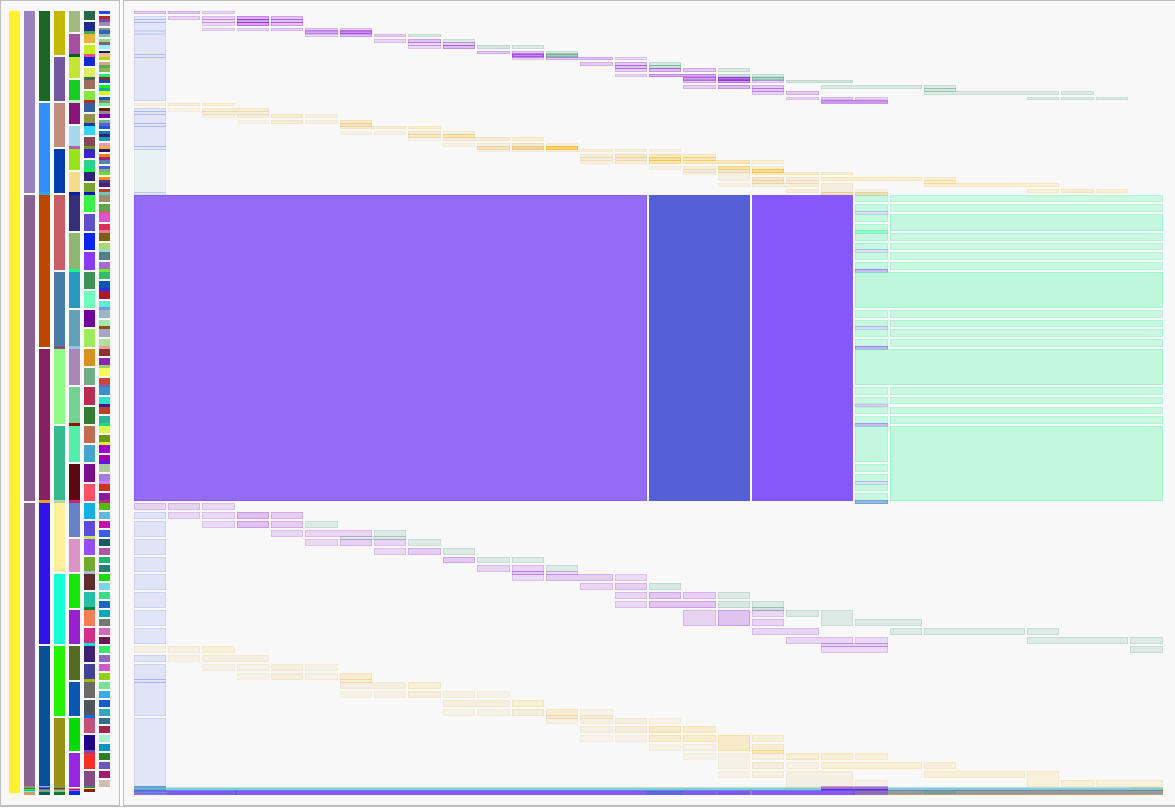
\includegraphics[width=\textwidth]{ocelotl/TaskView.png}
    \caption{Memory-gantt view of the naïve parallel matrix multiplication.}
    \label{fig:ocelotl-th0}
\end{figure}

\fig{ocelotl-th0} is a screenshot of \gls{Ocelotl} by thread visualization of \gls{Moca}.
We can see the hierarchy on the Y-axis, starting with the memory root, then three data structures.
The X-axis represent temporal evolution.
For more readability of the trace, we have set one color per thread independently from the type of access, thread zero is blue, one is green, two read, three orange and four violet.

From this view, we see clearly that blue accesses occurs only during the initialization phase except for a small data structure on the bottom of the figure.
Therefore we can see that the thread~$0$ is the master thread doing the initialization.
Moreover, the master thread also access to some private data (the small structures in the bottom).
Among these data, we can find a pid array used to wait the end of the slave threads.
We can confirm that by filtering the accesses to show only the accesses done by thread~$0$.
Or by zooming on the initialization phase.

During the rest of the execution, two data structures are accessed diagonally over the time, which means linearly.
Furthermore, the colors confirms that two threads are sharing each series of accesses.
The data structure in the middle is intensively accessed by every threads, as a result all the accesses are aggregated.

It seems that, at the two third of the execution, we can see a change of colors in the middle data structure.
Additionally, it seems that at the same time the violet thread has completed his work and does not access the memory anymore.

\begin{figure}[htb]
    \centering
    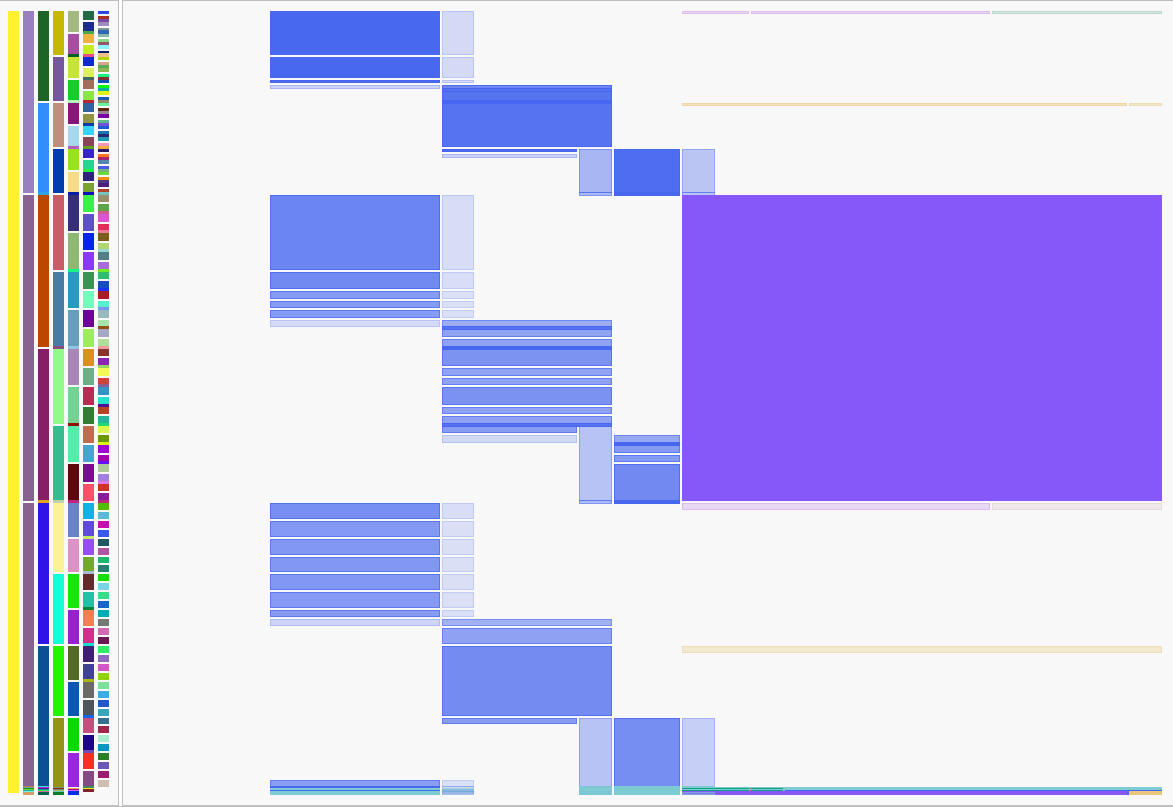
\includegraphics[width=\textwidth]{ocelotl/TaskView-zoom-init.png}
    \caption{Memory-gantt view of the naïve parallel matrix multiplication ,
    initialization}
    \label{fig:ocelotl-th1}
\end{figure}

Now let's zoom on the initialization step.
The result is shown in \fig{ocelotl-th1}.
We can see that, during the initialization phase, only the master thread is working.
We can identify a three diagonal patterns happening at the same time, it correspond to the matrix initialization.
The private data structures in the bottom also appears during the initialization.
Finally, we see that as soon as the thread~$0$ has finished to initialize the data structure, the other four threads start working.

\begin{figure}[htb]
    \centering
    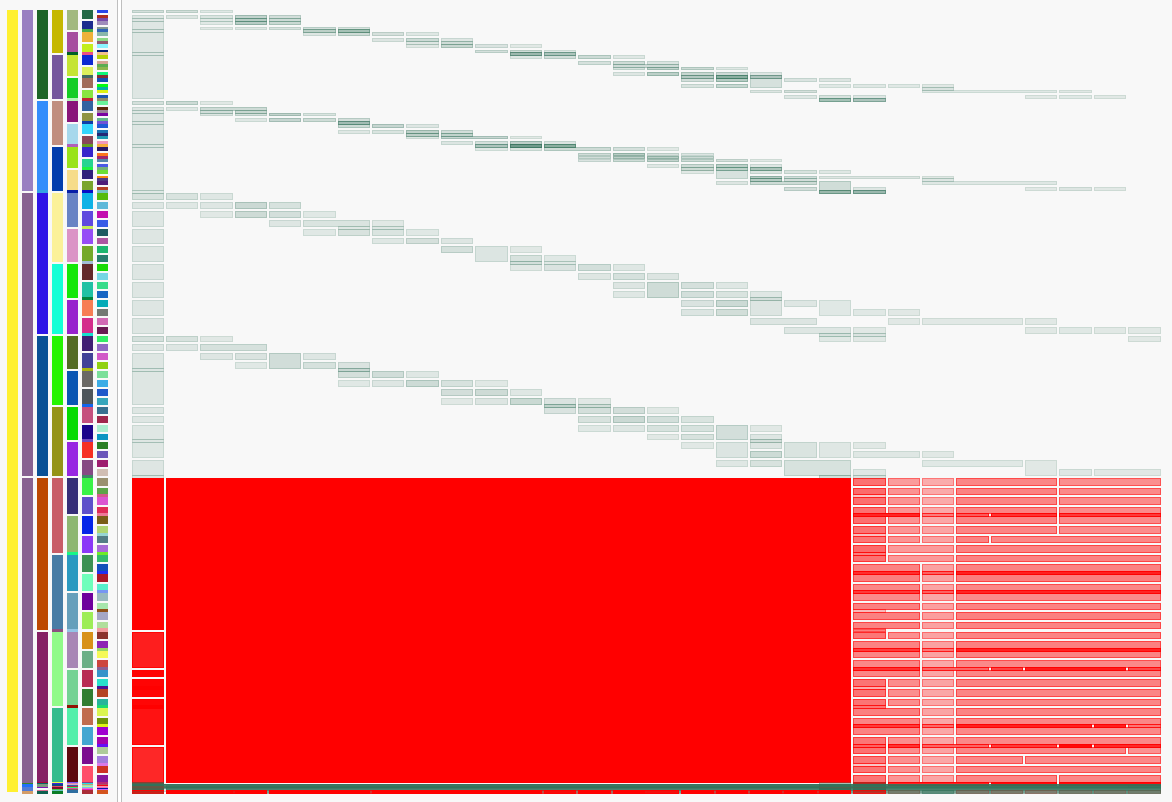
\includegraphics[width=\textwidth]{ocelotl/Sharing.png}
    \caption{Cartography view of the naïve parallel matrix multiplication.}
    \label{fig:ocelotl-carto0}
\end{figure}

In the previous view there were four access type per threads (private / shared, reads / writes) which means $20$ different access types.
To make the trace more readable, we had to reduce the number of colors and stop distinguishing private access from shared and reads from writes.
The global view that is designed to highlight sharing only provides for event types independently from the number of threads.
Therefore, it is easier to identify sharing patterns with this view.
\fig{ocelotl-carto0} shows this visualization of our example traces.
We can see that the trace looks like the previous one except that the order of the data structures is different.
Blue accesses are privates and reds are shared.
Dark colors are for writes while light ones means reads.
From this view, we can see that most accesses seems to be reads and except for the matrix B (on the bottom) they are all private.
Still the visualization is aggregated, at this point it is interesting to zoom in the middle of the execution and desegregate the trace as much as possible.

\begin{figure}[htb]
    \centering
    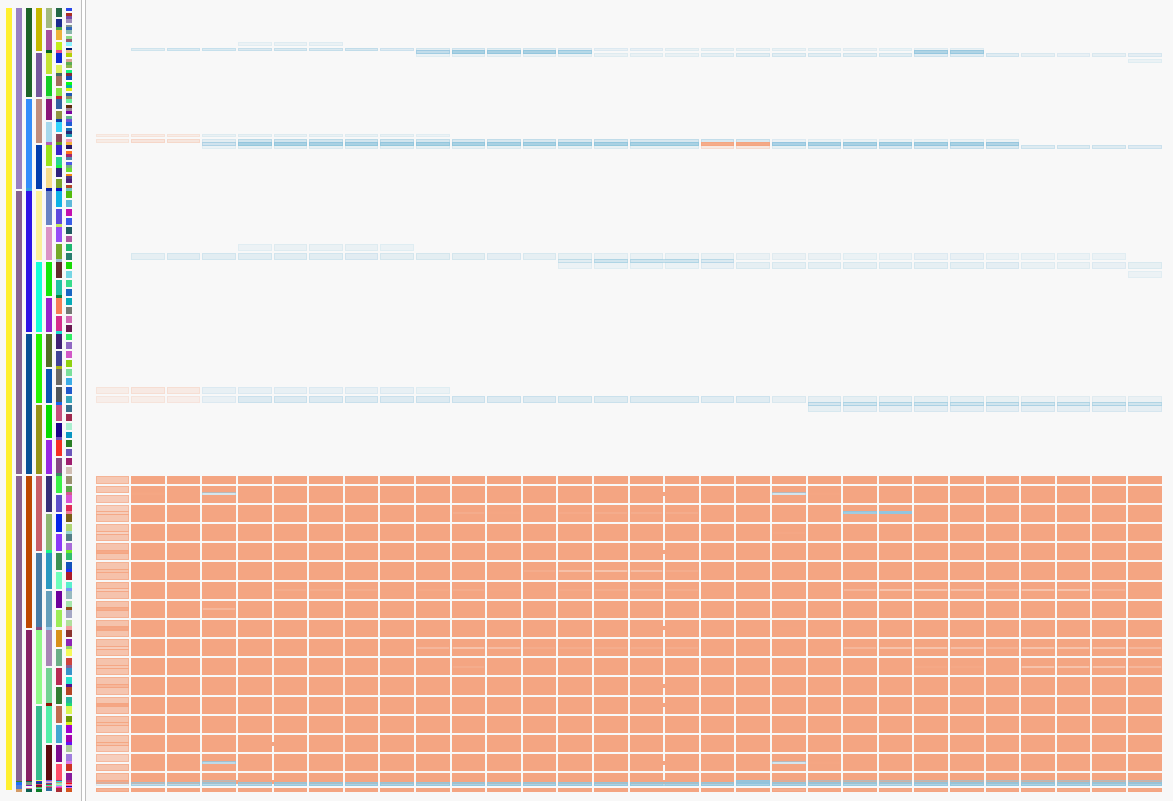
\includegraphics[width=\textwidth]{ocelotl/Sharing-zoom.png}
    \caption{Cartography view of the naïve parallel matrix multiplication, computing phase.}
    \label{fig:ocelotl-Carto-zoom}
\end{figure}

By focusing on the middle of the execution and setting $p$ to zero, we obtain the \fig{ocelotl-Carto-zoom}.
It is important to note that the trace is still aggregate due to the microscopic model of the trace.
This aggregation explains the fact that we still see small, regular, blocks of accesses.
We cannot identify a clear pattern on the bottom matrix, however, we can see a few private (blue) accesses appearing from time to time in this data structure.
The access on this matrix seem dense and not designed to fit in a cache.
This density of accesses is coherent with the behavior expected.
Indeed the matrix by is accessed column first by all the threads.
Due to the representation of 2D matrices in \texttt{C}, each access of each thread on B is separated from $sz$ doubles.
Hence \gls{Ocelotl} groups almost everything in a huge chunks of access on all the matrices.
We can also see in this figure that shared (orange) accesses appears regularly on the two other data structures which is also coherent with the expected behavior.

\subsection{Discussion}


\begin{itemize}
    \item Able to identify different patterns here
    \item Visu per thread
        \begin{itemize}
            \item Not scalable (need to adjust colors for each thread one by one)
        \end{itemize}
    \item Data structures not scalable
    \item No contexctual info on data structures
    \item Switch loose filters and zooms
    \item Computations slow: here small matrix needs 5 to 10 minutes to generate visu
    \item Selection based on addresses extremly slow (too much EPs) and not scalable
    \item Need something more scalable and flaxible hence programmatic approach\ldots
\end{itemize}

Although we were able to visualize all the inefficient patterns in the example described previously, we were not completely convinced of the visualization based on \gls{Ocelotl}.
Indeed, the first limitation comes from the fact that \gls{Framesoc} trace description is quite static and does not permit to change the event producers.
As a result we had to generate three traces (virtual addresses, physical addresses and by threads) to provide different visualizations.
This means that if we spot an interesting pattern in a visualization and want to look at it from another point of view, we need to reload the whole trace and  which breaks the flow of trace analysis.
Indeed \gls{Ocelotl} initial computations are slow as it requires to compare all possible partitions.
Additionally, by doing so we loose all filtering and zoom done on the previous trace.

Another limit of this approach is that it is hard to identify (name) the data structure.
Furthermore selecting only a set of data structure is slow as \gls{Framesoc} is not designed for handling as much event producers as we have with memory traces.
Finally meta data about there size or number of accesses are impossible to visualize.

To conclude, these visualization are interesting and enables identification classic mistakes.
Yet it seems that in the end \gls{Ocelotl} tool is no well suited for memory traces.
Therefore we should try a more dynamic approach that permit to change the point of view easily.

\section{Programmatic exploration}
\label{sec:visu-second}

The main drawback of using a generic visualization tool for analyzing \gls{Moca} traces come from the difficulty to switch the perspective from which we visualize the data.
This limitation comes from the static representation of the trace as a two dimensional entity.
Hence, a more programmatic approach may enable to work closer to the data and ease this point of view switch.
In \gls{R}, data are usually stored in huge dataframes, each row of a dataframe represent one observation and each column give the value of a parameter or a measure for this observation.
While this representation has a significant memory footprint, it ease switching point of view, as the same dataframe can represent several measures.
For these reason, we analyzed several traces with \gls{R}.
For more reproducibility, we store the evolution of our work in an \gls{Org-mode} labbook, as described in~\cite[Chapter~4, p~54]{Stanisic15Reproducible}, and available online at:\\
\url{https://github.com/dbeniamine/Moca\_visualization}.

While this approach is extremely flexible, it is not user friendly.
Indeed it requires to know how to write efficient \gls{R} code, how to use \gls{Org-mode} and Emacs and to read the labbook before doing an analysis.
Anyway, after a few analysis we obtained a basic procedure to analyze traces (parsing, transforming data, showing some generic visualization) from which we can adapt each step to the trace.
For instance we might want to ignore some parts of the trace very soon to focus on some data structures, or after analyzing one plot we might think of another representation of data that might be meaningful in this case.

\subsection{Design}

Our analysis converged very quickly to a classical yet adaptable analysis pipeline:
\begin{enumerate}
    \item Parsing: reading \gls{Moca} traces (to which we have applied the sharing detection written for \gls{Framesoc} and depicted in \fig{sharing-detection})
        and representing the data in a \gls{R} friendly way.
        At the end of this step, we have two dataframes, the main one contains all the accesses, and the other one the list of data structures.
    \item Creating simplified data frames: At this point, the main dataframe contains a set of accesses where shared access appears one time for each thread involved in the sharing as described in \fig{sharing-detection}.
        We can aggregate all theses accesses, reducing the size of the main dataframe.
    \item Retrieving the mapping between structures and pages: this step is the most costly one, but can be speed it up by several means:
        \begin{itemize}
            \item During the parsing step, we can easily compute the minimum and maximum address that are in a structure and ignore all accesses out of theses bounds.
            \item As there are significantly less data structures than memory addresses, we can do the mapping by applying on the data frame representing the structures, a function that returns a vector with one entry per line of the main data frame.
                When this function is applied, each data structures adds it names to the addresses that belongs to it.
                In the end we just have to add this vector as a column of the main data frame.
        \end{itemize}
    \item Predefined plots: Finally we can present some predefined  plots, the three first are inspired from \gls{Tabarnac} ones and show the size of data structures, the number of accesses, and amount of sharing.
        At this point it is trivial to focus on the data structures that have enough accesses with one line of \gls{R} code.
        Then we present a cartography view of the density of accesses or of sharing by data structures and by type of accesses.
    \item Zoom and modify plots: at this point it is possible to zoom or focus on some data structures by selecting subsets of the main dataframe.
        Furthermore, we can easily change the axes of the plots, show other metrics, do some conditional zoom on specific part of the trace \ldots
\end{enumerate}

\subsection{Results and discussion}

\begin{figure}[htb]
    \centering
    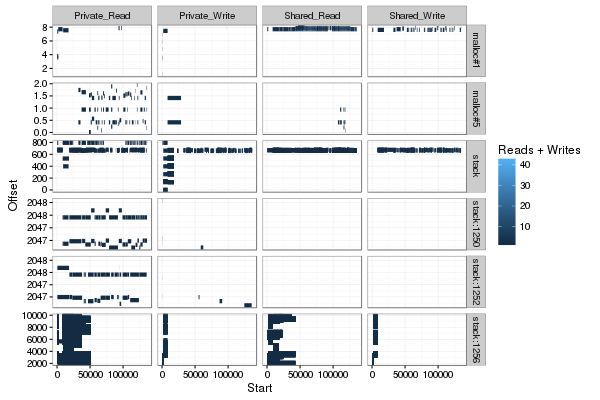
\includegraphics[width=\textwidth]{labbook/intensity_Rw_dgetrf}
    \caption{Visualization of the memory access of the dgetrf kernel from ffplas-ffpack.}
    \label{fig:dgetrf-intensity}
\end{figure}

We illustrate our visualization with the \emph{dgetrf} kernel from the fflas-ffpack~\cite{group16FFLASFFPACK} compiled against the OpenBlas~\cite{Chothia16OpenBlas}.
This trace was collected on a machine from the Edel cluster which hardware was presented in \tbl{hw-moca}.

\fig{dgetrf-intensity} shows for each data structures\footnote{
    A few almost unused data structures have been filtered out to make the image more readable.}
    the number of accesses per page over the time.
Furthermore we differentiate four types of access: \texttt{PrivateRead}, \texttt{PrivateWrites}, \texttt{SharedRead} and \texttt{SharedWrites}.

For each structures, some accesses seemed to appear private and shared at the same time which is not possible.
Nevertheless, by zooming on a small part of the execution were able to confirm that those access are interleaved and never of both types at the same time.
This means that several threads are working on data very close and often do actually share some pages.

From this visualization we can see that two of the stacks (1252 and 1250) are always used privately.
Furthermore the data structure malloc\#5 seems to be used mostly privately and only very rarely read in a shared way.
These three structures seems also to be accessed mostly linearly, hence they should not be subject to memory optimization.

\lstinputlisting[caption={R code to focus on interesting data structures.}, label=lst:R-zoom,float=htb]{code/zoom.R}

At this point, it is interesting to focus on these three data structures and ignore the others, we can do this with the simple line of code displayed in \lstr{R-zoom}.
Additionally, we can look at the amount of sharing instead of the number of axis just by changing the \emph{y} parameter of the plot.

\begin{figure}[htb]
    \centering
    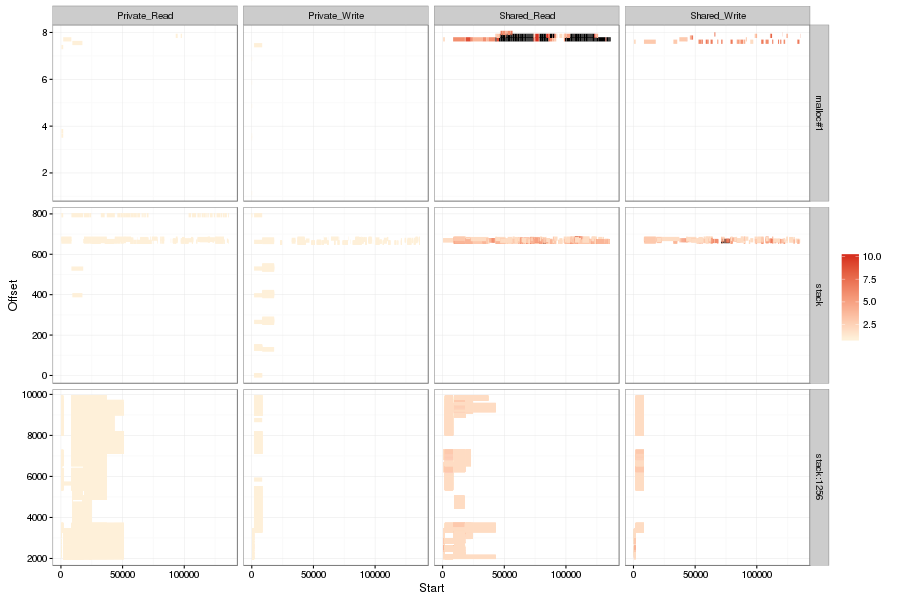
\includegraphics[width=\textwidth]{labbook/intensity_Share_dgetrf_zoom}
    \caption{Visualization of the memory access of the dgetrf kernel from ffplas-ffpack, zoom on the three interesting data structures.}
    \label{fig:dgetrf-share-zoom}
\end{figure}

We can see in \fig{dgetrf-share-zoom} that the sharing patterns are very similar to the access patterns.
The three other data structures present different and interesting memory access patterns.
First the malloc\#1 structure is very small and accessed intensively in a shared way, during all the execution and always on the same page.
We can presume that this data structure contains information about the threads status that must be updated quite often, maybe it is used for thread scheduling.
Second the stack 1256 is only used during the first third of the execution and written only at the beginning and in parallel.
For a generic data structure, this parallel initialization could probably have been designed to distribute first touch on the \gls{NUMA} nodes of the machine, still on a stack it seems quite unusual.
Last but not least, a small part of the main stack is accessed in read and write mode and in a shared way during all the execution.
This pattern means that threads are probably organized in a master / slave way, where the master thread allocates data in its stack (not dynamic allocation).
This might be problematic on \gls{NUMA} machines as the stack is statically allocated and thus cannot be allocated explicitly on some node.
It would be interesting to zoom on the beginning of the execution to check if the initialization of this part of the stack is correctly spread around the thread or not.
If not, Linux will allocate each page on the memory bank of the master thread independently of the re partition of the data between the threads.

After discussing these results with some of the developers of the fflas-ffpack, it appears that the observed patterns can be due to the OpenBlas library and might be complex to improve.
Yet an interesting thing to do would be to compare these traces, with the trace of the same kernel but compiled against the \gls{MKL}.
Indeed there are some performance differences between the two library that are hard to explain with traditional profiling tools as the \gls{MKL} code is proprietary.
Therefore, memory traces might help understanding the underlying algorithms.

In the end, this approach ease the exploration of \gls{Moca} traces, provided that we know a minimum of \gls{R} code.
Moreover, while \gls{Framesoc} and \gls{Ocelotl} can be easily used by an end user without the our intervention, at the time of the writing, this programmatic approach requires to read at least a part of the labbook to understand how to do the analysis.
Additionally, we had some troubles to analyze some traces from Lulesh \gls{OpenMP} and \gls{SOFA}.
Indeed these applications generates thousands of call to the malloc functions (hundreds of thousands for Lulesh).
Hence, retrieving the mapping page to data structure was extremely slow or nearly impossible without merging some data structures.
In the end it appears that we need both a more user friendly tool, and a way to add a priori knowledge of the developers in the parsing step to filter out uninteresting data.

\subsection{Generic trace visualization tool}

Programmatic exploration of traces is extremely powerful but not user friendly.
We describe here an hypothetical, generic trace viewer based on \gls{R} that should make trace exploration more user friendly.
We only provide some principles of design and interaction that results from our experiment while trying to analyze traces with \gls{R}.

\begin{figure}[htb]
    \centering
    %!TEX encoding=UTF-8 Unicode

% Layers
\pgfdeclarelayer{background}
\pgfdeclarelayer{foreground}
\pgfsetlayers{background,main,foreground}

\definecolor{TraceCol}{HTML}{B2ABD2}
\definecolor{UserCol}{HTML}{FDB863}
\definecolor{ViewerCol}{HTML}{E66101}
\definecolor{EntityCol}{HTML}{5E3C99}

\tikzstyle{entity} = [drawed box=EntityCol]
\tikzstyle{userbox} = [filled box=UserCol,shape=circle]

\tikzstyle{trace}  = [-latex,TraceCol,thick]
\tikzstyle{view} =   [-latex,ViewerCol,thick]

%\newlength{\cornerlength}
%\setlength{\cornerlength}{.1}

\tikzset{
  basic box/.style = {
    shape = rectangle,
    draw,
    text centered,
    text width=5em,
    },
  rounded box/.style={
    basic box,
    rounded corners,
  },
  drawed box/.style ={
    rounded box,
    draw = #1,},
  filled box/.style = {
    rounded box,
    draw  = #1,
    fill  = #1,
  },
  concrete box/.style = {
    shape = rectangle,
    text centered,
    text width=5em,
    draw  = #1,
    fill  = #1,
  },
    corner/.style={
      shape=rectangle,
      fill=white,
      alias=this,
      append after command = {
          \pgfextra{
              \begin{pgfonlayer}{foreground}
                % Borders of the corner
                \draw [] (this.south west) -- (this.south east);
                \draw [] (this.south west) -- (this.north west);
                \draw [] (this.north west) -- (this.south east);
                % Borders of the main rectangle
                \draw [] (#1.north west)   -- (this.north west);
                \draw [] (#1.north west)   -- (this.north west);
                \draw [] (#1.north west)   -- (#1.south west);
                \draw [] (#1.south west)   -- (#1.south east);
                \draw [] (#1.south east)   -- (this.south east);
              \end{pgfonlayer}
            }
      }
  },
  file/.style ={
      shape = rectangle,
      text centered,
      fill = TraceCol,
      minimum height = 5.5em,
      text width = 3.5em,
      append after command = {
            \pgfextra{\let\TikZlastnode\tikzlastnode}
                node [corner=\TikZlastnode, anchor=north east] (corner-\TikZlastnode) at
                (\TikZlastnode.north east){}
          }
  },
  fileT/.style ={
      file,
      fill =TraceCol,
  },
  fileV/.style ={
      file,
      fill =ViewerCol,
  },
  header node/.style = {
    %Minimum Width = header nodes,
    font          = \strut\large,%\ttfamily,
  %  text depth    = +0pt,
    fill          = #1,
    text         = white,
    draw},
    header/.style n args={4}{%
    inner ysep = +1.7em,
    append after command = {
      \pgfextra{\let\TikZlastnode\tikzlastnode}
      node [header node=#2,#4] (header-\TikZlastnode) at (\TikZlastnode.#3) {#1}
      %node %[span = (\TikZlastnode)(header-\TikZlastnode)]
       % at (fit bounding box) (h-\TikZlastnode) {}
    }
  },
  hv/.style = {to path = {-|(\tikztotarget)\tikztonodes}},
  vh/.style = {to path = {|-(\tikztotarget)\tikztonodes}},
  fat blue line/.style = {ultra thick, blue}
}
\begin{tikzpicture}[font=\small,scale=1]


    \node [userbox] (user) at (0,0) {User};

    \node[filled box=ViewerCol] (shell) at (3,0) {\textbf{Shell:} R and Commands (pop, zoom, filtrate)};

    \node[filled box=ViewerCol] (stack) at (5.5,0) {R dataframe Stack};

    \node [fileT] (f0) at (8,0) {Main Data};
    \node [fileT] (f1) at (10,0) {Meta Data};
    \node [fileT] (f2) at (9,-2.5) {Other File};

    \begin{pgfonlayer}{background}
        \node[entity,fit=(f0) (f1) (f2),%
        header={Trace}{EntityCol}{north}{}] (trace) {};
    \end{pgfonlayer}

    \node [filled box=TraceCol]   (rqf) at (6, -6) {Required files};
    \node [concrete box=TraceCol] (pc) at  (9, -6) {Parsing code};
    \node [concrete box=TraceCol] (pp) at  (7.5,-8) {Predefined plots};

    \begin{pgfonlayer}{background}
        \node[entity,fit=(rqf) (pc) (pp),%
        header={Configuration}{EntityCol}{south}{}] (config) {};
    \end{pgfonlayer}


    \begin{pgfonlayer}{background}
        \node[entity,draw=ViewerCol,fit=(shell) (stack),%
            header={Viewer}{ViewerCol}{north}{}] (viewer) {};
    \end{pgfonlayer}

    \path[trace]  (rqf.north) edge[out=90,in=-90] node[pos=.3,above] {Defines} (trace.south);

    \path[view] (viewer.south) edge[out=-90,in=180] node[pos=.3,right] {Loads} (config.west);

    \draw[view] ($(user.east)+(-.1,.2)$) -- ($(viewer.west)+(0,.2)$);
    \draw[view] ($(viewer.west)+(0,-.2)$) -- ($(user.east)+(-.1,.-.2)$);

\end{tikzpicture}
% vim: et si sta lbr  sw=4 ts=4 spelllang=en_us

    \caption{Description of a R based hypothetical generic trace viewer.}
    \label{fig:generic-viewer}
\end{figure}

The main components and interactions of our hypothetical tool are presented in \fig{generic-viewer}.
To be generic this tool is split in two parts: the viewer itself is quite minimalist, it contains a few predefined commands for interacting with data (zoom, filters \ldots), with the dataframe stack that will be described later and do predefined actions (parse, show some plot).
The second part is the configuration and should be provided by the developer of the tracing tool.
This configuration defines six things:
\begin{itemize}
    \item The code required to implement the trace interaction commands (zoom, filter etc.).
    \item Optionally some code to define some specific commands.
    \item The files that constitute the trace.
    \item The code used to do the parsing steps.
    \item Some breakpoints that can be used to insert code during parsing.
    \item The code used to provide the main predefined plots.
\end{itemize}

Another important idea is that the tool should conserve a \emph{dataframe stack} which means that the users will work on a small set of dataframes, and every modification to a dataframe (except if specified otherwise) should generate a copy.
While this means a considerable memory footprint, it enables rolling back if a step of aggregation (for instance) loose too much information.
Moreover, the first step of the analysis often consists in filtering data to focus on the most meaningful part of the trace.
Hence, only the first copies will have an important impact on the memory footprint.

The users would have two ways to interact with this tool: use builtin commands (or commands defined by the tool), or \gls{R} code.
These two usage are not incompatible.
At any step the users can see the code of the next step that they want to run and modify it or execute it.
A natural workflow would be to start analyzing the trace with the commands provided with the trace, and if necessary, start running \gls{R} code to generate new visualizations or filter data.
In the end, the user would be able to export the code of the new visualization to improve the original configuration.

\section{Discussions}
\label{sec:visu-cncl}

Visualizing \gls{Moca} traces is a complex task.
Indeed these traces are spread over five dimensions: time, addresses (virtual or physical), threads, \gls{CPU} location and access type.
Furthermore, the address space is quite large and we are mostly interest on some specific patterns.
Therefore, we first used \gls{Ocelotl} to analyze these traces.
This tool is designed to aggregate traces in a meaningful way, trying to provide a good trade-off between information lost and data reduction.
Moreover it is implemented as a \gls{Framesoc} tool.
\gls{Framesoc} is a generic trace manager, that provide a simple \gls{API} to import traces from virtually any tools.
Importing \gls{Moca} traces inside \gls{Framesoc} is also interesting as it provides easy filtering and zoom on the traces.
Still, \gls{Framesoc} considers that a trace has two dimensions: time and event producers, it is hard to represent the complexity of \gls{Moca} traces in it.
As a result, we had to generate several different \gls{Framesoc} traces while importing one \gls{Moca} trace.
The main drawback of this workaround is that switching traces inside \gls{Framesoc} means loosing all zooms and filters along with the caches and the results of the aggregated views computed by \gls{Ocelotl}.
In the end this approach enable the visualization of small traces, yet the cost of changing the perspective is too high and makes the interaction too slow to be usable.

Our second approach to analyze these trace was more programmatic, we use \gls{R} and saved all our attempts in a labbook.
While this is not user friendly at all, \gls{R} is a powerful tool and it enables more complex visualization.
We are able to do efficient and complex zoom with \gls{R} selection operators.
To make this analysis reproducible by users not familiar with \gls{R}, it would be interesting to develop a generic viewer build upon predefined \gls{R} visualization.
Such viewer should (at least) provide the two following feature: simple (non \gls{R}) zoom and filtering and a dataframe stack so the users can rollback if they discard some useful informations.

Another approach that have not been studied during this thesis would be to analyze traces automatically.
Such analysis would have to detect memory patterns and possibly and highlight parts of code that should be improved.
A memory pattern is an interaction between threads inside a memory area over a short laps of time.
Yet, defining such a pattern in a more specific way is a hard task.

For any approach, it appears that the developers knowledge is useful to focus the analysis on the interesting parts.
Therefore we need a way to use this knowledge during the analysis and as soon as possible to reduce the amount of data we need to analyze.
Nerveless, we have seen in \chap{perf} that they might not know all the source of performance issues.
In the end, this knowledge can be used to focus the analysis but it is important to also have a global visualization of the trace, to spot issue that would have been missed by the developers.
Hence the two approaches described in this chapter can be used in a complementary way.

% vim: et si sta lbr  sw=4 ts=4 spelllang=en_us
